%% Template para TCC na classe IFBATCC
%% versao 1.0
%% (c) 2021 Antônio Cleber de Sousa Araújo
%% https://github.com/cleberaraujo/ifbatcc.git
%% versao 1.1
%% (c) 2023 Leandro Costa Souza
%% https://github.com/ifbasaj/tcc-template.git

%% Carrega a classe ifbatcc
%% Opcoes: * Idiomas
%%           pt   - português (padrao)
%%           en   - inglês
%%         * Tipos de Trabalhos (pelos graus de formação)
%%           tec  - para TCC de cursos tecnólogos (padrão)
%%           bsc  - para monografias de graduação
%%           msc  - para dissertações de mestrado
%%           qual - exame de qualificação de mestrado
%%           prop - exame de qualificação de doutorado
%%           phd  - para teses de doutorado
%%         * Cursos do IFBA/SAJ
%%           ads  - Análise e Desenvolvimento de Sistemas
%%           rde  - Redes de Computadores (padrão)
%%           mul  - Produção Multimídia
%%         * Mídia
%%           scr  - para versão eletrônica (PDF) / consulte o guia do usuário
%%         * Estilo
%%           classic - estilo original a la TAOCP (deprecated)
%%           std     - novo estilo a la CUP (padrão)
%%         * Paginação
%%           oneside - para impressão em face única
%%           twoside - para impressão em frente e verso (padrão)
\documentclass[tec, ads, scr, classic, a4paper]{ifbatcc}
\usepackage[utf8]{inputenc}
\usepackage{nomencl}
\makenomenclature


%% Preâmbulo:
%% coloque aqui o seu preambulo LaTeX, i.e., declaração de pacotes,
%% (re)definicoes de macros, medidas, etc.

%% Identificação:

% Nome da biblioteca - usado na ficha catalográfica
% default: Biblioteca do IFBA Campus Santo Antônio de Jesus
\library{Biblioteca do IFBA \textit{Campus} Santo Antônio de Jesus}

% Programas de pós graduação
% e.g. \program{Pós graduação em Redes Linux}
%\program{Curso Superior em Tecnologia}

% Titulo do TCC
% e.g. \title{Redes de Computadores em SAJ}
\title{TITULO DO TRABALHO}

% Data da defesa
% e.g. \date{19 de fevereiro de 2021}
\date{DATA DA DEFESA}

% Autor
% e.g. \author{José da Silva}
\author{NOME DO AUTOR}

% Orientador(a)
% Opcao: [f] - para orientadora do sexo feminino
% e.g. \adviser[f]{Profa. Dra. Maria Santos}
\adviser{NOME DO(DA) ORIENTADOR(A)}

% Orientador(a)
% Opcao: [f] - para orientadora do sexo feminino
% e.g. \coadviser{Prof. Dr. Pedro Pedreira}
% Comente se não se aplicar
%\coadviser{NOME DO(DA) CO-ORIENTADOR(A)}

%% Inicio do documento
\begin{document}

%% Catalogação do TCC
%% IFBA/SAJ - Sigla do curso - Número ordinal de trabalhos dete curso
\ifbafrontpage{IFBA/SAJ-ADS-XXXX}

%%
%% Parte pre-textual
%%
\frontmatter

\ifbapresentationpage
% Se seu trabalho for uma dissertação de mestrado, use a linha acima
%\presentationpage
% Se for qualificação, use \presentationpage

% Ficha catalográfica
\authorcitationname{SEU NOME EM CITACOES} % e.g. Sobrenome, Nome e sobrenome do meio
\advisercitationname{NOME DO SEU ORIENTADOR EM CITACOES} % e.g. Araújo, Antônio Cleber de Sousa
\coadvisercitationname{NOME DO SEU CO-ORIENTADOR EM CITACOES} % e.g. Silva, João Santos
\catalogtype{TIPO DE TRABALHO} % e.g. ``Tese (doutorado)''
\catalogtopics{TOPICOS PARA FICHA CATALOGRAFICA} % e.g. ``1. Complexidade Estrutural. 2. Engenharia de Software''
\catalogcdd{NUMERO CDD} % e.g. ``CDD 20.ed. XXX.YY'' (esse número será passado pela biblioteca)
\catalogingsheet

%% Termo de aprovação
%% Composição da Banca Avaliadora
\approvalsheet{Santo Antônio de Jesus - BA, DIA de MES de ANO}{
  \comittemember{Profa. Dra. Professora 1}{Universidade XYZ}
  \comittemember{Prof. Dr. Professor 2}{Universidade 123}
  \comittemember{Profa. Dra. Professora 3}{Universidade ABC}
}

% Dedicatória
% Comente para ocultar
\begin{dedicatory}
DIGITE A DEDICATÓRIA AQUI
\end{dedicatory}

% Agradecimentos
% Se preferir, crie um arquivo a parte e o inclua via \include{}
\acknowledgements
DIGITE OS AGRADECIMENTOS AQUI

% Epigrafe
% Comente para ocultar
% e.g.
%  \begin{epigraph}[Tarde, 1919]{Olavo Bilac}
%  última flor do Lácio, inculta e bela,\\
%  És, a um tempo, esplendor e sepultura;\\
%  Ouro nativo, que, na ganga impura,\\
%  A bruta mina entre os cascalhos vela.
%  \end{epigraph}
\begin{epigraph}[NOTA]{AUTOR}
DIGITE AQUI A CITACAO
\end{epigraph}

% Resumo em Portugues
% Se preferir, crie um arquivo separado e o inclua via \include{}
\resumo
DIGITE O RESUMO AQUI
% Palavras-chave do resumo em Portugues
\begin{keywords}
DIGITE AS PALAVRAS-CHAVE AQUI
\end{keywords}

% Resumo em Inglês
% Se preferir, crie um arquivo separado e o inclua via \include{}
\abstract
% Palavras-chave do resumo em Inglês
\begin{keywords}
DIGITE AS PALAVRAS-CHAVE AQUI
\end{keywords}

% Sumario
% Comente para ocultar
\tableofcontents

% Lista de figuras
% Comente para ocultar
\listoffigures

% Lista de tabelas
% Comente para ocultar
\listoftables

\newcommand{\listadesiglasname}{LISTA DE ABREVIATURAS E SIGLAS}
\renewcommand{\nomname}{\listadesiglasname}
\renewcommand{\nomlabel}[1]{\textbf{#1}\hfil}
\printnomenclature[3cm]
\cleardoublepage
\nomenclature{ADS}{Análise e Desenvolvimento de Sistemas}

%%
%% Parte textual
%%
\mainmatter

% Recomendados criar cada capitulo em um arquivo separado, por exemplo
% "capitulo1.tex", "capitulo2.tex", ... "capituloN.tex" e depois
% inclui-los com:
% \include{capitulo1}
% \include{capitulo2}
% ...
% \include{capituloN}
%
% Importante: Use \xchapter ao invés de \chapter, conforme exemplo abaixo.
%\xchapter{Introdução}{Este é o primeiro capítulo, no qual eu conto toda a história deste trabalho.}


%%%%%%%%%%%%%%%%%%%%%%%%%%%%%%%%%%%%%%%%%%%%%%%%%%%%%%
\xchapter{Introdução}{Um breve resumo deste capítulo}
\label{cap:introducao}
%%%%%%%%%%%%%%%%%%%%%%%%%%%%%%%%%%%%%%%%%%%%%%%%%%%%%%

Lorem ipsum dolor sit amet, consectetur adipiscing elit. Praesent ac tellus turpis. Donec vitae lorem odio. Sed luctus vestibulum libero eget pellentesque. Vivamus in mi turpis. Donec molestie feugiat sollicitudin. Nam et eleifend tortor. Cras lacinia, magna in tristique consequat, urna lorem placerat odio, id viverra mi nulla nec sem. Ut imperdiet, felis a hendrerit imperdiet, velit metus eleifend diam, ut convallis neque augue vitae leo. Morbi condimentum rhoncus faucibus. Fusce elit justo, semper lobortis blandit sed, lacinia et ligula. Pellentesque elit magna, vestibulum vitae adipiscing in, tincidunt eu erat. Nullam eu lectus vel nunc eleifend consectetur. Phasellus faucibus blandit nisi, eget fermentum erat tincidunt et. Aliquam ullamcorper varius nunc, nec eleifend dolor porttitor eu. Etiam eget nunc eu erat facilisis consequat sed accumsan urna. Nam vitae eros et justo iaculis gravida in sed nisl. Donec auctor gravida ipsum. Morbi sed ipsum tortor, quis ornare purus.

Nulla facilisi. Praesent nec massa nulla, interdum lobortis orci. Integer convallis porttitor congue. Etiam lectus ipsum, iaculis eu malesuada malesuada, scelerisque semper est. In convallis ipsum lacus, at dapibus velit. Praesent semper diam eget eros ultrices quis elementum libero cursus. Aliquam erat volutpat. Nunc a lectus augue, id sagittis neque. Aliquam dignissim tempus sem ut pellentesque. Nulla libero orci, elementum vel malesuada mattis, adipiscing sed lorem. Cras lacinia elit vel magna mollis ut congue elit faucibus. Duis ornare mollis est, quis hendrerit neque convallis in.

Donec at leo sed nisl varius iaculis. Sed ullamcorper nisl sit amet metus sollicitudin quis cursus elit imperdiet. Donec vel ante sed elit tempor hendrerit. Quisque commodo neque a ante tempor rhoncus. Proin purus metus, interdum mattis elementum quis, mollis et felis. Curabitur id nibh ac sapien porta pellentesque vel nec sapien. Duis ullamcorper consectetur elit, eleifend tincidunt leo adipiscing a. Cras nunc quam, sodales sit amet semper at, pharetra quis libero. Vestibulum posuere risus sed ante interdum tempor. Sed nec enim lorem, eu ultrices nisl. Maecenas cursus lacus non metus convallis cursus. Cras egestas feugiat libero, quis luctus justo mattis ut. Proin vitae magna et purus convallis blandit ut sed risus. Nulla vel ligula massa, vel interdum tortor. Integer sit amet eros sit amet lectus suscipit adipiscing. Aenean sagittis diam eu orci porttitor luctus.

Sed sed elit eu ante malesuada aliquet. Nunc quis quam turpis, accumsan faucibus sapien. Nam eget sem velit, id eleifend elit. Phasellus auctor egestas libero a adipiscing. Integer convallis, nunc sed tincidunt sollicitudin, augue diam accumsan risus, sit amet lacinia neque quam at lorem. Quisque ac rhoncus mauris. Donec felis odio, consequat vitae pretium ullamcorper, blandit id lorem. Morbi nec tellus vitae velit eleifend bibendum at vel eros. Sed quis enim urna. Cras placerat ultricies ipsum, sed tempor lorem placerat vitae. Morbi tellus leo, blandit eget feugiat nec, bibendum egestas erat. Mauris lobortis congue vestibulum. Nunc ultricies arcu in neque hendrerit convallis. Phasellus facilisis dictum nulla vel iaculis. Donec in adipiscing tellus. Aliquam non turpis neque. Nam in velit nec tortor gravida convallis. Vivamus tincidunt eros quis elit ultricies at adipiscing urna tempor. Donec posuere, ante pulvinar laoreet adipiscing, eros nulla pharetra nulla, vel rutrum elit est vitae ligula.

Phasellus urna nulla, laoreet in imperdiet a, porttitor eu nibh. Phasellus ac arcu magna, sit amet dapibus eros. Maecenas eget metus vitae leo feugiat lobortis ac quis tortor. Pellentesque habitant morbi tristique senectus et netus et malesuada fames ac turpis egestas. Pellentesque vel augue metus. Quisque fringilla, arcu ut fringilla consectetur, mauris tellus euismod sem, in vehicula est leo vel nisi. Praesent sapien ligula, malesuada eget hendrerit ac, aliquet nec turpis. Cum sociis natoque penatibus et magnis dis parturient montes, nascetur ridiculus mus. Nulla facilisi. Mauris commodo elementum elit, fermentum placerat nulla iaculis nec. Vestibulum neque dui, cursus at pharetra eu, sollicitudin eget justo. In id dignissim augue. Fusce interdum malesuada ipsum, non aliquet quam auctor eget. Curabitur turpis libero, pharetra ut cursus porta, pellentesque vitae magna. Cras porttitor interdum nisl.

Lorem ipsum dolor sit amet, consectetur adipiscing elit. Praesent ac tellus turpis. Donec vitae lorem odio. Sed luctus vestibulum libero eget pellentesque. Vivamus in mi turpis. Donec molestie feugiat sollicitudin. Nam et eleifend tortor. Cras lacinia, magna in tristique consequat, urna lorem placerat odio, id viverra mi nulla nec sem. Ut imperdiet, felis a hendrerit imperdiet, velit metus eleifend diam, ut convallis neque augue vitae leo. Morbi condimentum rhoncus faucibus. Fusce elit justo, semper lobortis blandit sed, lacinia et ligula. Pellentesque elit magna, vestibulum vitae adipiscing in, tincidunt eu erat. Nullam eu lectus vel nunc eleifend consectetur. Phasellus faucibus blandit nisi, eget fermentum erat tincidunt et. Aliquam ullamcorper varius nunc, nec eleifend dolor porttitor eu. Etiam eget nunc eu erat facilisis consequat sed accumsan urna. Nam vitae eros et justo iaculis gravida in sed nisl. Donec auctor gravida ipsum. Morbi sed ipsum tortor, quis ornare purus.



%%%%%%%%%%%%%%%%%%%%%%%%%%%%%%%%%%%%%%%%%%%%%%%
\xchapter{Revisão Bibliográfica}{Neste capítulo eu apresento todo o material que eu estudei durante a elaboração do trabalho.}
\label{cap:revisao}
%%%%%%%%%%%%%%%%%%%%%%%%%%%%%%%%%%%%%%%%%%%%%%%


Lorem ipsum dolor sit amet, consectetur adipiscing elit. Praesent ac tellus turpis. Donec vitae lorem odio. Sed luctus vestibulum libero eget pellentesque. Vivamus in mi turpis. Donec molestie feugiat sollicitudin. Nam et eleifend tortor. Cras lacinia, magna in tristique consequat, urna lorem placerat odio, id viverra mi nulla nec sem. Ut imperdiet, felis a hendrerit imperdiet, velit metus eleifend diam, ut convallis neque augue vitae leo. Morbi condimentum rhoncus faucibus. Fusce elit justo, semper lobortis blandit sed, lacinia et ligula. Pellentesque elit magna, vestibulum vitae adipiscing in, tincidunt eu erat. Nullam eu lectus vel nunc eleifend consectetur. Phasellus faucibus blandit nisi, eget fermentum erat tincidunt et. Aliquam ullamcorper varius nunc, nec eleifend dolor porttitor eu. Etiam eget nunc eu erat facilisis consequat sed accumsan urna. Nam vitae eros et justo iaculis gravida in sed nisl. Donec auctor gravida ipsum. Morbi sed ipsum tortor, quis ornare purus \cite{demeyer2008}.

Nulla facilisi. Praesent nec massa nulla, interdum lobortis orci. Integer convallis porttitor congue. Etiam lectus ipsum, iaculis eu malesuada malesuada, scelerisque semper est. In convallis ipsum lacus, at dapibus velit. Praesent semper diam eget eros ultrices quis elementum libero cursus. Aliquam erat volutpat. Nunc a lectus augue, id sagittis neque. Aliquam dignissim tempus sem ut pellentesque. Nulla libero orci, elementum vel malesuada mattis, adipiscing sed lorem. Cras lacinia elit vel magna mollis ut congue elit faucibus. Duis ornare mollis est, quis hendrerit neque convallis in.


%% Exemplo de Figura
\begin{figure}[!htb]
\centerline{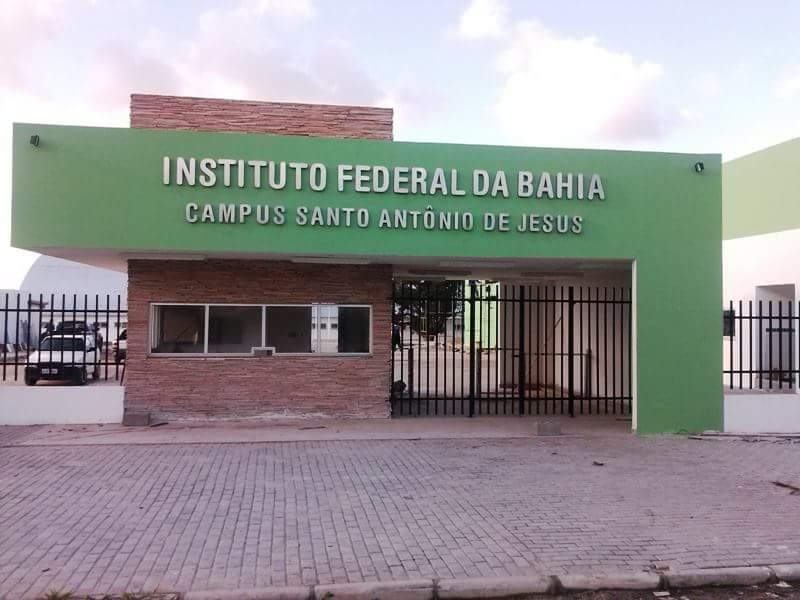
\includegraphics[width=.8\textwidth]{ifba_saj.jpeg}}
\caption{Exemplo de Imagem utilizando uma foto do IFBA SAJ.}
\label{fig:ifba}
\end{figure}

Como usar a imagem no texto? A Figura~\ref{fig:ifba} apresenta uma foto do IFBA \textit{Campus} Santo Antônio de Jesus, datada de 14 de maio de 2021.

Donec at leo sed nisl varius iaculis. Sed ullamcorper nisl sit amet metus sollicitudin quis cursus elit imperdiet. Donec vel ante sed elit tempor hendrerit. Quisque commodo neque a ante tempor rhoncus. Proin purus metus, interdum mattis elementum quis, mollis et felis. Curabitur id nibh ac sapien porta pellentesque vel nec sapien. Duis ullamcorper consectetur elit, eleifend tincidunt leo adipiscing a. Cras nunc quam, sodales sit amet semper at, pharetra quis libero. Vestibulum posuere risus sed ante interdum tempor. Sed nec enim lorem, eu ultrices nisl. Maecenas cursus lacus non metus convallis cursus. Cras egestas feugiat libero, quis luctus justo mattis ut. Proin vitae magna et purus convallis blandit ut sed risus. Nulla vel ligula massa, vel interdum tortor. Integer sit amet eros sit amet lectus suscipit adipiscing. Aenean sagittis diam eu orci porttitor luctus.

Sed sed elit eu ante malesuada aliquet. Nunc quis quam turpis, accumsan faucibus sapien. Nam eget sem velit, id eleifend elit. Phasellus auctor egestas libero a adipiscing. Integer convallis, nunc sed tincidunt sollicitudin, augue diam accumsan risus, sit amet lacinia neque quam at lorem. Quisque ac rhoncus mauris. Donec felis odio, consequat vitae pretium ullamcorper, blandit id lorem. Morbi nec tellus vitae velit eleifend bibendum at vel eros. Sed quis enim urna. Cras placerat ultricies ipsum, sed tempor lorem placerat vitae. Morbi tellus leo, blandit eget feugiat nec, bibendum egestas erat. Mauris lobortis congue vestibulum. Nunc ultricies arcu in neque hendrerit convallis. Phasellus facilisis dictum nulla vel iaculis. Donec in adipiscing tellus. Aliquam non turpis neque. Nam in velit nec tortor gravida convallis. Vivamus tincidunt eros quis elit ultricies at adipiscing urna tempor. Donec posuere, ante pulvinar laoreet adipiscing, eros nulla pharetra nulla, vel rutrum elit est vitae ligula.

%% Exemplo de Tabela
%% Foi proposital colocar a legenda com o mesmo nome acima da tabela
%% Vejam como mesclar células e colocar fundo ;)
\begin{table}[h]
\begin{center}
\caption{Alguns livros na biblioteca do IFBA Campus SAJ}
\label{tabela:livros}
\begin{adjustbox}{max width=\textwidth}
\begin{tabular}{clccc}
\toprule
\textbf{Nº} & \multicolumn{1}{c}{\textbf{Título}} & \textbf{Autor} & \textbf{Área} & \textbf{Quantidade} \\ 
\toprule 
                   1   & Redes e a Internet                 & Fulano         & Redes                          & 3                  \\ \midrule
                   2   & Programação é vida                 & Beltrano       & ADS                            & 4                  \\ \midrule
  \multirow{2}{*}{3}   & \multirow{2}{*}{Multimídia 100\%}  & Sicrana        & \multirow{2}{*}{Multimídia}    & \multirow{2}{*}{5} \\ 
                       &                                    & Telânio        &                                & \\   
\bottomrule
\end{tabular}
\end{adjustbox}
\end{center}
\end{table}

Phasellus urna nulla, laoreet in imperdiet a, porttitor eu nibh. Phasellus ac arcu magna, sit amet dapibus eros. Maecenas eget metus vitae leo feugiat lobortis ac quis tortor. Pellentesque habitant morbi tristique senectus et netus et malesuada fames ac turpis egestas. Pellentesque vel augue metus. Quisque fringilla, arcu ut fringilla consectetur, mauris tellus euismod sem, in vehicula est leo vel nisi. Praesent sapien ligula, malesuada eget hendrerit ac, aliquet nec turpis. Cum sociis natoque penatibus et magnis dis parturient montes, nascetur ridiculus mus. Nulla facilisi. Mauris commodo elementum elit, fermentum placerat nulla iaculis nec. Vestibulum neque dui, cursus at pharetra eu, sollicitudin eget justo. In id dignissim augue. Fusce interdum malesuada ipsum, non aliquet quam auctor eget. Curabitur turpis libero, pharetra ut cursus porta, pellentesque vitae magna. Cras porttitor interdum nisl \cite{raymond1999}.

A Tabela \ref{tabela:livros} mostra, de forma fictícia, alguns livros contidos na bilioteca do IFBA \textit{Campus} SAJ. Os mesmos podem ser utilizados para leitura local, como estão disponíveis para empréstimo.

%%
%% Parte pós-textual
%%
\backmatter

% Apêndices
% Comente se não houver apêndices
\appendix

% É aconselhável criar cada apêndice em um arquivo separado, exemplo
% "apendice1.tex", "apendice.tex", ... "apendiceM.tex" e depois
% inclui--los com:
% \include{apendice1}
% \include{apendice2}
% ...
% \include{apendiceM}


% Bibliografia
% É aconselhável utilizar o BibTeX a partir de um arquivo, digamos "biblio.bib".
% Para ajuda na criação do arquivo .bib e utilização do BibTeX
\bibliographystyle{abntex2-alf}
\bibliography{biblio}

% Colofon
% Inclui uma pequena nota com referencia a classe IFBATCC
% Comente para omitir
\colophon

%% Fim do documento
\end{document}